\chapter{Part H: Treasury Bonds/Risky Bonds}
Developer: Joseph Perez

\noindent Validator: Aloke Mukherjee


%DEVELOPER WRITES THIS PART --->

\section{Requirements}
In this section we design an object that take into account the characteristic of a bond (either a treasury bond or a risky bond) mainly in order to price it.

Usually on the contract of a bond are specified the maturity, the date of the first coupon, the date of issue, the annual value of coupons, their frequency, the faceamount and the daycount convention. Those are information are required to create a bond object.




\section{Design }
Treasury bond and risky bond are similar except that to be priced we use a yield curve for the T-bond and a credit curve for the risky bond. As those bonds are closely tied with those curves we decided to incorporate them into the constructor.
We designed one class for T-bonds and another one for risky bonds. Both inherits from a generic class bond.

\section{Choices}
As a bond price is a decreasing function of its yield to maturity, We find the yield to maturity for a given price with the recursive Newton-Raphson algorithm.
%<any important design choices you made, e.g. data structures, class hierarchy, algorithm, etc. and a justification for the decision>

\section{Methods}
We implemented several methods :
\begin{itemize}
	\item getCashflow returns an array of cash flows with their dates
	\item quotedPrice which is the present value of the cash flows
	\item fairvalue, the sum of the quotedPrice and the interest accrual
	\item yieldToMaturity, duration and convexity
\end{itemize}
At time $t_i$ we have the cash flow $CF_i=facevalue*coupon/frequency$ and if $t_i$ is the time of the last coupon $CF_i=coupon/frequency + facevalue$, the discount factor between 0 and $t_i$ is $DF_i$ is given by the yield/curve.
Let $t'$ be the time between the reception of the last coupon (if there had one else the date of issue) and today and $t''$ be the date of the reception of the next coupon and the time between the reception of the last coupon (if there had one else the date of issue). Let also $y$ be the yield to maturity.
\bes
quotedPrice &=& \sum_i CF_i * DF_i\\
fairvalue &=& quotedPrice + facevalue*coupon*t'/t''\\
duration &=& \frac{\sum_i CF_ie^{-yt_i}t_i}{fairvalue}\\
convexity &=& \frac{\sum_i CF_ie^{-yt_i}t_i^2}{fairvalue}
\ens
\section{Unit tests}

\begin{figure}
\begin{center}
        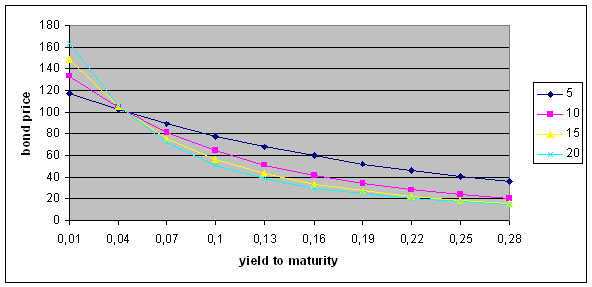
\includegraphics[width=12cm]{bondprice.jpg}
        \caption{bond prices for different maturities}
\end{center}
\end{figure}

The chart had been drawn with bonds having the following specificities
\begin{center}
\begin{tabular}{|c|c|}
\hline
bond & treasury bond\\
coupon & $4.5 \%$ \\
daycount & ACT/365\\
frequence &  semianual\\
faceamount & 100 \\
\hline
\end{tabular}
\end{center}
The values we get are in accord with the Treasury bond provided. We can't claim we found exactly the same price because we didn't have the yield curve at that time.

%<short descriptions of each subtest>

\section{Performance}
Most of methods implies simple computations so it would be difficult to improve the efficiency of this class. We use Newton-Raphson algorithm, the comment on this algorithm in the section Volatility Surface holds.
%<how can the performance of this component be sped up by 100%?>

%VALIDATOR WRITES THIS PART --->

\section{Validation}
\subsection{Approach}

We used inputs of table 5.7 'Calculation of duration' of \underline{Options, Futures and Other derivatives} (fourth ed.) by John Hull to compare our duration to theirs. Both duration matched.



%<i.e. what alternate method was used to validate the results - if this required a lot of code then similar outline as above should apply>

%\subsection{Pitfalls}

%<i.e. what bugs were found>
